%% bare_conf.tex
%% V1.3
%% 2007/01/11
%% by Michael Shell
%% See:
%% http://www.michaelshell.org/
%% for current contact information.
%%
%% This is a skeleton file demonstrating the use of IEEEtran.cls
%% (requires IEEEtran.cls version 1.7 or later) with an IEEE conference paper.
%%
%% Support sites:
%% http://www.michaelshell.org/tex/ieeetran/
%% http://www.ctan.org/tex-archive/macros/latex/contrib/IEEEtran/
%% and
%% http://www.ieee.org/

%%*************************************************************************
%% Legal Notice:
%% This code is offered as-is without any warranty either expressed or
%% implied; without even the implied warranty of MERCHANTABILITY or
%% FITNESS FOR A PARTICULAR PURPOSE!
%% User assumes all risk.
%% In no event shall IEEE or any contributor to this code be liable for
%% any damages or losses, including, but not limited to, incidental,
%% consequential, or any other damages, resulting from the use or misuse
%% of any information contained here.
%%
%% All comments are the opinions of their respective authors and are not
%% necessarily endorsed by the IEEE.
%%
%% This work is distributed under the LaTeX Project Public License (LPPL)
%% ( http://www.latex-project.org/ ) version 1.3, and may be freely used,
%% distributed and modified. A copy of the LPPL, version 1.3, is included
%% in the base LaTeX documentation of all distributions of LaTeX released
%% 2003/12/01 or later.
%% Retain all contribution notices and credits.
%% ** Modified files should be clearly indicated as such, including  **
%% ** renaming them and changing author support contact information. **
%%
%% File list of work: IEEEtran.cls, IEEEtran_HOWTO.pdf, bare_adv.tex,
%%                    bare_conf.tex, bare_jrnl.tex, bare_jrnl_compsoc.tex
%%*************************************************************************

% *** Authors should verify (and, if needed, correct) their LaTeX system  ***
% *** with the testflow diagnostic prior to trusting their LaTeX platform ***
% *** with production work. IEEE's font choices can trigger bugs that do  ***
% *** not appear when using other class files.                            ***
% The testflow support page is at:
% http://www.michaelshell.org/tex/testflow/



% Note that the a4paper option is mainly intended so that authors in
% countries using A4 can easily print to A4 and see how their papers will
% look in print - the typesetting of the document will not typically be
% affected with changes in paper size (but the bottom and side margins will).
% Use the testflow package mentioned above to verify correct handling of
% both paper sizes by the user's LaTeX system.
%
% Also note that the "draftcls" or "draftclsnofoot", not "draft", option
% should be used if it is desired that the figures are to be displayed in
% draft mode.
%
\documentclass[conference]{IEEEtran}
% Add the compsoc option for Computer Society conferences.
%
% If IEEEtran.cls has not been installed into the LaTeX system files,
% manually specify the path to it like:
% \documentclass[conference]{../sty/IEEEtran}

\IEEEoverridecommandlockouts
%\graphicspath{{/figs/}}
% Turkce karakterler icin.
%\usepackage[turkish]{babel}
\usepackage[utf8]{inputenc} % Kullanılan encodinge göre utf8 yerine latin5 de yazılabilir.
\usepackage[T1]{fontenc}



% Some very useful LaTeX packages include:
% (uncomment the ones you want to load)


% *** MISC UTILITY PACKAGES ***
%
%\usepackage{ifpdf}
% Heiko Oberdiek's ifpdf.sty is very useful if you need conditional
% compilation based on whether the output is pdf or dvi.
% usage:
% \ifpdf
%   % pdf code
% \else
%   % dvi code
% \fi
% The latest version of ifpdf.sty can be obtained from:
% http://www.ctan.org/tex-archive/macros/latex/contrib/oberdiek/
% Also, note that IEEEtran.cls V1.7 and later provides a builtin
% \ifCLASSINFOpdf conditional that works the same way.
% When switching from latex to pdflatex and vice-versa, the compiler may
% have to be run twice to clear warning/error messages.






% *** CITATION PACKAGES ***
%
\usepackage{cite}
% cite.sty was written by Donald Arseneau
% V1.6 and later of IEEEtran pre-defines the format of the cite.sty package
% \cite{} output to follow that of IEEE. Loading the cite package will
% result in citation numbers being automatically sorted and properly
% "compressed/ranged". e.g., [1], [9], [2], [7], [5], [6] without using
% cite.sty will become [1], [2], [5]--[7], [9] using cite.sty. cite.sty's
% \cite will automatically add leading space, if needed. Use cite.sty's
% noadjust option (cite.sty V3.8 and later) if you want to turn this off.
% cite.sty is already installed on most LaTeX systems. Be sure and use
% version 4.0 (2003-05-27) and later if using hyperref.sty. cite.sty does
% not currently provide for hyperlinked citations.
% The latest version can be obtained at:
% http://www.ctan.org/tex-archive/macros/latex/contrib/cite/
% The documentation is contained in the cite.sty file itself.






% *** GRAPHICS RELATED PACKAGES ***
%
\ifCLASSINFOpdf
  \usepackage[pdftex]{graphicx}
  % declare the path(s) where your graphic files are
  \graphicspath{{../figs/}}
  % and their extensions so you won't have to specify these with
  % every instance of \includegraphics
  \DeclareGraphicsExtensions{.pdf,.jpeg,.png}
\else
  % or other class option (dvipsone, dvipdf, if not using dvips). graphicx
  % will default to the driver specified in the system graphics.cfg if no
  % driver is specified.
  % \usepackage[dvips]{graphicx}
  % declare the path(s) where your graphic files are
  % \graphicspath{{../eps/}}
  % and their extensions so you won't have to specify these with
  % every instance of \includegraphics
  % \DeclareGraphicsExtensions{.eps}
\fi
% graphicx was written by David Carlisle and Sebastian Rahtz. It is
% required if you want graphics, photos, etc. graphicx.sty is already
% installed on most LaTeX systems. The latest version and documentation can
% be obtained at:
% http://www.ctan.org/tex-archive/macros/latex/required/graphics/
% Another good source of documentation is "Using Imported Graphics in
% LaTeX2e" by Keith Reckdahl which can be found as epslatex.ps or
% epslatex.pdf at: http://www.ctan.org/tex-archive/info/
%
% latex, and pdflatex in dvi mode, support graphics in encapsulated
% postscript (.eps) format. pdflatex in pdf mode supports graphics
% in .pdf, .jpeg, .png and .mps (metapost) formats. Users should ensure
% that all non-photo figures use a vector format (.eps, .pdf, .mps) and
% not a bitmapped formats (.jpeg, .png). IEEE frowns on bitmapped formats
% which can result in "jaggedy"/blurry rendering of lines and letters as
% well as large increases in file sizes.
%
% You can find documentation about the pdfTeX application at:
% http://www.tug.org/applications/pdftex





% *** MATH PACKAGES ***
%
\usepackage[cmex10]{amsmath}
% A popular package from the American Mathematical Society that provides
% many useful and powerful commands for dealing with mathematics. If using
% it, be sure to load this package with the cmex10 option to ensure that
% only type 1 fonts will utilized at all point sizes. Without this option,
% it is possible that some math symbols, particularly those within
% footnotes, will be rendered in bitmap form which will result in a
% document that can not be IEEE Xplore compliant!
%
% Also, note that the amsmath package sets \interdisplaylinepenalty to 10000
% thus preventing page breaks from occurring within multiline equations. Use:
%\interdisplaylinepenalty=2500
% after loading amsmath to restore such page breaks as IEEEtran.cls normally
% does. amsmath.sty is already installed on most LaTeX systems. The latest
% version and documentation can be obtained at:
% http://www.ctan.org/tex-archive/macros/latex/required/amslatex/math/


%Akciğer nodülü, etkileşimli öğrenme, hacimsel görüntü analizi


% *** SPECIALIZED LIST PACKAGES ***
%
%\usepackage{algorithmic}
% algorithmic.sty was written by Peter Williams and Rogerio Brito.
% This package provides an algorithmic environment fo describing algorithms.
% You can use the algorithmic environment in-text or within a figure
% environment to provide for a floating algorithm. Do NOT use the algorithm
% floating environment provided by algorithm.sty (by the same authors) or
% algorithm2e.sty (by Christophe Fiorio) as IEEE does not use dedicated
% algorithm float types and packages that provide these will not provide
% correct IEEE style captions. The latest version and documentation of
% algorithmic.sty can be obtained at:
% http://www.ctan.org/tex-archive/macros/latex/contrib/algorithms/
% There is also a support site at:
% http://algorithms.berlios.de/index.html
% Also of interest may be the (relatively newer and more customizable)
% algorithmicx.sty package by Szasz Janos:
% http://www.ctan.org/tex-archive/macros/latex/contrib/algorithmicx/




% *** ALIGNMENT PACKAGES ***
%
\usepackage{array}
% Frank Mittelbach's and David Carlisle's array.sty patches and improves
% the standard LaTeX2e array and tabular environments to provide better
% appearance and additional user controls. As the default LaTeX2e table
% generation code is lacking to the point of almost being broken with
% respect to the quality of the end results, all users are strongly
% advised to use an enhanced (at the very least that provided by array.sty)
% set of table tools. array.sty is already installed on most systems. The
% latest version and documentation can be obtained at:
% http://www.ctan.org/tex-archive/macros/latex/required/tools/


\usepackage{mdwmath}
\usepackage{mdwtab}
% Also highly recommended is Mark Wooding's extremely powerful MDW tools,
% especially mdwmath.sty and mdwtab.sty which are used to format equations
% and tables, respectively. The MDWtools set is already installed on most
% LaTeX systems. The lastest version and documentation is available at:
% http://www.ctan.org/tex-archive/macros/latex/contrib/mdwtools/


% IEEEtran contains the IEEEeqnarray family of commands that can be used to
% generate multiline equations as well as matrices, tables, etc., of high
% quality.


%\usepackage{eqparbox}
% Also of notable interest is Scott Pakin's eqparbox package for creating
% (automatically sized) equal width boxes - aka "natural width parboxes".
% Available at:
% http://www.ctan.org/tex-archive/macros/latex/contrib/eqparbox/





% *** SUBFIGURE PACKAGES ***
\usepackage[tight,footnotesize]{subfigure}
% subfigure.sty was written by Steven Douglas Cochran. This package makes it
% easy to put subfigures in your figures. e.g., "Figure 1a and 1b". For IEEE
% work, it is a good idea to load it with the tight package option to reduce
% the amount of white space around the subfigures. subfigure.sty is already
% installed on most LaTeX systems. The latest version and documentation can
% be obtained at:
% http://www.ctan.org/tex-archive/obsolete/macros/latex/contrib/subfigure/
% subfigure.sty has been superceeded by subfig.sty.



%\usepackage[caption=false]{caption}
%\usepackage[font=footnotesize]{subfig}
% subfig.sty, also written by Steven Douglas Cochran, is the modern
% replacement for subfigure.sty. However, subfig.sty requires and
% automatically loads Axel Sommerfeldt's caption.sty which will override
% IEEEtran.cls handling of captions and this will result in nonIEEE style
% figure/table captions. To prevent this problem, be sure and preload
% caption.sty with its "caption=false" package option. This is will preserve
% IEEEtran.cls handing of captions. Version 1.3 (2005/06/28) and later
% (recommended due to many improvements over 1.2) of subfig.sty supports
% the caption=false option directly:
%\usepackage[caption=false,font=footnotesize]{subfig}
%
% The latest version and documentation can be obtained at:
% http://www.ctan.org/tex-archive/macros/latex/contrib/subfig/
% The latest version and documentation of caption.sty can be obtained at:
% http://www.ctan.org/tex-archive/macros/latex/contrib/caption/




% *** FLOAT PACKAGES ***
%
%\usepackage{fixltx2e}
% fixltx2e, the successor to the earlier fix2col.sty, was written by
% Frank Mittelbach and David Carlisle. This package corrects a few problems
% in the LaTeX2e kernel, the most notable of which is that in current
% LaTeX2e releases, the ordering of single and double column floats is not
% guaranteed to be preserved. Thus, an unpatched LaTeX2e can allow a
% single column figure to be placed prior to an earlier double column
% figure. The latest version and documentation can be found at:
% http://www.ctan.org/tex-archive/macros/latex/base/



%\usepackage{stfloats}
% stfloats.sty was written by Sigitas Tolusis. This package gives LaTeX2e
% the ability to do double column floats at the bottom of the page as well
% as the top. (e.g., "\begin{figure*}[!b]" is not normally possible in
% LaTeX2e). It also provides a command:
%\fnbelowfloat
% to enable the placement of footnotes below bottom floats (the standard
% LaTeX2e kernel puts them above bottom floats). This is an invasive package
% which rewrites many portions of the LaTeX2e float routines. It may not work
% with other packages that modify the LaTeX2e float routines. The latest
% version and documentation can be obtained at:
% http://www.ctan.org/tex-archive/macros/latex/contrib/sttools/
% Documentation is contained in the stfloats.sty comments as well as in the
% presfull.pdf file. Do not use the stfloats baselinefloat ability as IEEE
% does not allow \baselineskip to stretch. Authors submitting work to the
% IEEE should note that IEEE rarely uses double column equations and
% that authors should try to avoid such use. Do not be tempted to use the
% cuted.sty or midfloat.sty packages (also by Sigitas Tolusis) as IEEE does
% not format its papers in such ways.





% *** PDF, URL AND HYPERLINK PACKAGES ***
%
%\usepackage{url}
% url.sty was written by Donald Arseneau. It provides better support for
% handling and breaking URLs. url.sty is already installed on most LaTeX
% systems. The latest version can be obtained at:
% http://www.ctan.org/tex-archive/macros/latex/contrib/misc/
% Read the url.sty source comments for usage information. Basically,
% \url{my_url_here}.

% *** Do not adjust lengths that control margins, column widths, etc. ***
% *** Do not use packages that alter fonts (such as pslatex).         ***
% There should be no need to do such things with IEEEtran.cls V1.6 and later.
% (Unless specifically asked to do so by the journal or conference you plan
% to submit to, of course. )


%\usepackage{multirow}
%\usepackage{array}
%\usepackage[lofdepth,lotdepth]{subfig}
\newcommand{\todo}[1]{{\noindent\color{red}\textsc{Todo}: #1}}
% correct bad hyphenation here
\hyphenation{sasa}


\begin{document}

\IEEEpubid{\makebox[\columnwidth]{978-1-5090-1679-2/16/\$31.00 ©2016 IEEE\hfill}
\hspace{\columnsep}\makebox[\columnwidth]{}}

%
% paper title
% can use linebreaks \\ within to get better formatting as desired
\title{Etkileşimli Öğrenme ile Akciğer Tomografi Hacim Taramalarında Nodül Tespiti\\
Interactive Learning Based Nodule Detection in CT Lung Volumes}

% author names and affiliations
% use a multiple column layout for up to three different
% affiliations
\author{\IEEEauthorblockN{İlker Çam, F. Boray Tek}
\IEEEauthorblockA{Bilgisayar Mühendisliği Bölümü, Işık Üniversitesi, İstanbul, Türkiye\\
{\{ilker.cam,boray.tek\}}@isikun.edu.tr}
}

% conference papers do not typically use \thanks and this command
% is locked out in conference mode. If really needed, such as for
% the acknowledgment of grants, issue a \IEEEoverridecommandlockouts
% after \documentclass

% for over three affiliations, or if they all won't fit within the width
% of the page, use this alternative format:
%
% use for special paper notices
%\IEEEspecialpapernotice{(Invited Paper)}




% make the title area
\maketitle

\begin{ozet}
Bu bildiride akciğer BT taramalarında otomatik nodül tespiti yapmak üzere geliştirdiğimiz yeni ve özgün bir yöntem sunulmaktadır. Önerdiğimiz yöntem, akciğer organına ve belirli bir nodül tipine bağlı kalmaksızın genelleştirilmiş bir yaklaşım sunmaktadır. Böylelikle akciğer bölütlemesine ihtiyaç duymamaktadır. Düşük doz radyasyonlu ve çeşitli tipte (katı ve kırık cam görünümlü, yüzeye ve damara ilişik) 10 mm'den küçük nodüllerden oluşan zorlu bir tarama kümesinde (Anode09) sınamalar yapılmıştır. Tarama başına ortalama 8 yanlış tespit için nodül tespit duyarlılığı \%52'dir. Yarışmada ilk altıya giren algoritmalarla karşılaştırılabilir düzeydedir.

%\boldmath
\end{ozet}
\begin{IEEEanahtar}
etkileşimli bölütleme, akciğer, nodül tespiti, bilgisayarlı tomografi
\end{IEEEanahtar}

\begin{abstract}
We present a novel method to automatically detect lung nodules in CT lung scans. Our method is generalized in the sense that it does not assume/depend a particular organ or a particular nodule type. hence it does not require an organ segmentation. We test our method in a challenging set (Anode09) that is comprised of low dose CT scans which include all types of nodules (solid, ground glass opacity, juxta-fissural, juxta-vascular) of less than 10mm in size. Our method produces \~8 false positives per scan for true positive rate of 52\%, which is comparable to the first 6 results from the contest.
%\boldmath
\end{abstract}
\begin{IEEEkeywords}
interactive segmentation, nodule detection, lung, computed tomography,
\end{IEEEkeywords}

% IEEEtran.cls defaults to using nonbold math in the Abstract.
% This preserves the distinction between vectors and scalars. However,
% if the conference you are submitting to favors bold math in the abstract,
% then you can use LaTeX's standard command \boldmath at the very start
% of the abstract to achieve this. Many IEEE journals/conferences frown on
% math in the abstract anyway.

% no keywords

% For peer review papers, you can put extra information on the cover
% page as needed:
% \ifCLASSOPTIONpeerreview
% \begin{center} \bfseries EDICS Category: 3-BBND \end{center}
% \fi
%
% For peerreview papers, this IEEEtran command inserts a page break and
% creates the second title. It will be ignored for other modes.
\IEEEpeerreviewmaketitle

\IEEEpubidadjcol

\section{GİRİŞ}

Kanser bütün dünyada ve ülkemizde giderek artan bir sağlık sorunudur. Globocan’ın \cite{ferlay2012} 184 ülkede ortaklaşa yaptığı araştırmalara göre, 2012’de toplam 14.1 milyon kanser teşhisi koyulmuş, 8 milyon insan hayatını kaybetmiştir. İnvasif olmaması nedeniyle özellikle akciğer ve kolon taramalarında kullanılan yöntemlerin başında bilgisayarlı \textbf{düşük dozlu} tomografi tarama gelmektedir. Modern bilgisayarlı tomografi (BT) cihazları yüksek çözünürlüklerde çalışarak 200-500 arasında kesit tarar. Radyografik okuma, hacimi oluşturan kesit imgeler arasında yukarı aşağı gezinerek hacimsel yapıyı kavramak için lokal değişimleri incelemeyi gerektirir. Bir radyoloğun tüm bir hacim taramasını incelemesi dikkate değer bir zaman almaktadır. Doğal olarak bu iş mühendislerin ilgisini çekmiş ve  bilgisayar destekli teşhis (BDT) algoritmaları geliştirmeye yöneltmiştir.

Kansere neden olabilecek nodüller görünüm (katı, yarı-katı, kırık cam), konumlanma (plevral, damara bitişik, izole gibi) ve büyüklük itibariyle farlılıklar gösterir. Büyük boyutlu (>~10mm) nodüllerin iyi huylu olup olmadıkları başka yöntemlerle araştırılabilir. Küçük boyutlu (<10mm) nodüllerin ise tespit edildiklerinde kayıt edilmeleri ve boyutlarının ölçülmesi gerekir. Radyologların özellikle küçük nodülleri tespit etme duyarlılığında ciddi farklılılar olduğu gözlenmiştir \cite{rubin2015}. Yine aynı çalışmada yardımcı okuyucu veya ikinci okuyucu olarak BDT kullanıldığı takdirde tespitte farklılıkların azaldığı gözlenmiştir. Bütün bunların yanında düşük dozlu tomografi taramalarda (<30mA) lezyonları belirlemek normal-yüksek dozlu taramalara göre daha zordur.

Bilgisayarlı tomografi tarama (BT) görüntülerinde lezyon tespiti, ölçümü ve sınıflandırmasını otomatik yapmayı amaçlayan yöntemler genellikle bir tek organı veya lezyonu hedef almaktadır. Bu tür yöntemler BT taramasında ilgili organı, örneğin akciğeri bölütleyecek bir ön-işlem ile başlar; aday vokselleri şekil, renk, vb niteliklerle tespit eden ikinci bir algoritma çalıştırılabilir; aday bileşenlerden öznitelikler çıkarılır; ve bir son sınıflandırıcı aday bileşenler içerisinde lezyonları tespit eder. Akciğer organı için katı nodülleri tespit eden/sayan algoritma, çok farklı görünümdeki bağırsak organında polip tespiti için kullanılamaz. Bunun yanında bir çok akciğer nodül tespit algoritması sadece katı veya yarı katı nodülleri tespit edebilir. Ortak veri setleri ile yapılan karşılaştırmalardaki hali hazırdaki algoritmaların yeterince genelleşmiş bir kullanılabilirliği yakalayamadığı; düşük radyasyon dozu ile taranmış hacimlerde ve küçük nodüllerde yeterince başarılı olmadığı gözlenmiştir \cite{anode09}. 

\begin{figure}
\centering
\subfigure[]{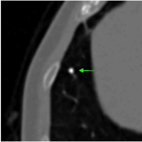
\includegraphics[scale=0.7]{figs/solid.png}}
\subfigure[]{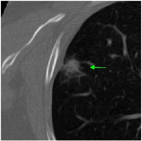
\includegraphics[scale=0.7]{figs/ggo.png}}
\caption{Örnek kümemizde yer alan iki farklı nodül örneği: a) katı ve izole bir nodül; b) kırık cam görünümlü nodül.}
\label{fig0}
\end{figure}

Bu çalışmada etkileşimli (interaktif) öğrenme ve bölütlemeden yola çıkarak BT hacimlerinde, organ bölütlemesine gerek duymayan, lezyonları şekil, konum gibi özelliklerle sınırlamayan bir nodül tespit yönteminin ön çalışması yapılmıştır. 
%Geliştirdiğimiz yöntemde 1) akciğer bölütlemesine ihtiyaç duyulmamaktadır; 2) tespit edilecek nodül şekli, konumu, veya tipi için bir ön kabullenme yapılmamıştır. Bu nedenlerle önerdiğimiz yöntem literatürde yer alan diğer nodül tespiti yaklaşımlarından oldukça farklıdır: kullanılabilirliği yüksek bir çerçeve yöntemdir. Yöntemimizde potansiyel lezyon pikselleri/vokselleri etkileşimli öğrenme ile öğrenmekte; tespit edilen adayları sınıflandırmak için özgün ve yine genel (jenerik) öznitelikler kullanmaktayız. Özniteliklerimiz radyologların inceleme metodlarından esinlenmiş ve farklı kesitler arasındaki diferansiyel bilgiyi yakalamaya yöneliktir.



\section{VERİ}\label{veriler}
Bu çalışmada kullandığımız veri, iki farklı kaynaktan derlenmiştir: Lung Image Database Consortium \cite{lidc2011} ve Anode09 \cite{anode09}. LIDC'den derlediğimiz 67 adet tarama (Veri 1) farklı doz aralıklarında (30mA-250mA), kesit kalınlığı 0.5-2.0 mm ve kesit sayısı 250-400 arasında değişmektedir. Toplamda 228 adet katı ve kırık cam görünümlü, yüzeye yapışık ve damara ilişmiş nödüller bulundurmaktadır. Anode09 yarışması veritabanından elde ettiğimiz 5 farklı düşük dozlu taramada (30mA), 1.0 mm kesit kalınlığında ve 300-500 kesit sayısında, toplamda 39 adet genellikle 5-10 mm arasında katı ve kırık cam görünümlü, yüzeye yapışık ve damara yapışık nödül bulundurmaktadır (Veri 2). Veri 1 kümesindeki nodüllerin bütün vokselleri, uzman radyologlar tarafından el ile işaretlenmiştir. Veri 2 kümesinde ise nodüllerin orta noktaları işaretlenmiştir. Anode09 yarışmasının değerlendirilmesi için, organizatörler tarafından derlenen 50 adet etiketsiz tarama (Veri 3), çalışmamızın sınanması için kullanılmıştır.
%Çalışmamızda, eğitim ve test setlerini tamamıyla ayrı tuttuğumuz bir yapı bulunmaktadır. İnteraktif öğrenme sürecinde kullandığımız eğitim seti, Şekil \ref{eq1}'de örneği gösterilen 55 adet ilgi bölgesinden oluşan taramalardır. Art işleme aşamasında örnek geliştirilmesi amacıyla 77 adet ve deney sürecinde 5 adet akciğer taramaları içermektedir. \ref{ground truth}
%Çalışmada kullanılan veri kümesi, nodül işaretlemeleriyle birlikte tamamı genele açıktır.



\section{YÖNTEM}
Şekil \ref{figflow} görülebileceği gibi yöntemimiz dört ana parçadan oluşmaktadır. 1) Etkileşimli öğrenme ile eğitilmiş piksel/voksel sınıflandırıcının voksel olasıklıklarını hesaplaması; 2) Piksellerden bağlı bileşenlerin hesaplanarak aday objelerin belirlenmesi; 3) Özniteliklerin hesaplanması; 4) Rastgele karar ormanı ile objelerin nodül ve nodül-olmayan sınıflara ayrılması.

\begin{figure*}[tb!]
\centering
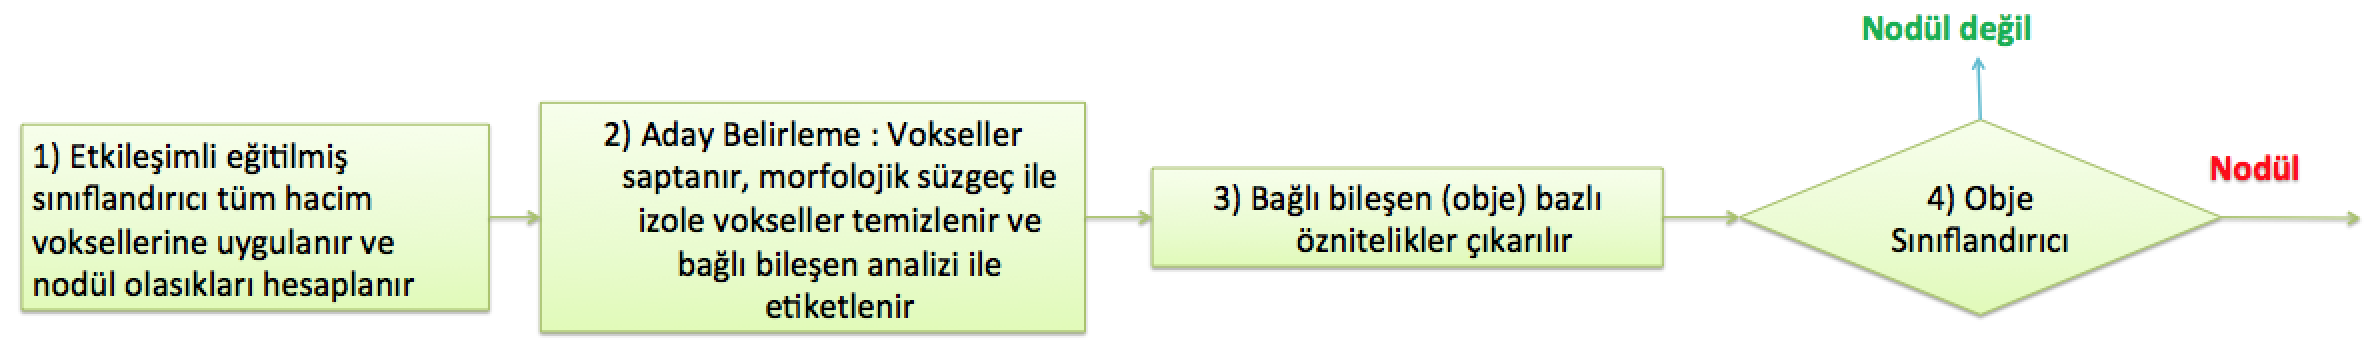
\includegraphics[width=\textwidth]{figs/flow.png}
\caption{Nodül tespit yöntemimizin akış diyagramı}
\label{figflow}
\end{figure*}

\subsection{Etkileşimli Öğrenme}\label{ilastik}
Otomatik lezyon tespiti algoritmaları genellikle bölütleme aşaması ile başlar. Tomografi görüntülerinin bölütlenmesi, hedef alınan organa bağlı olarak özel yöntemler gerektirir. Bu çalışmada organa yönelik bir ön işleme gereksinimi kaldırmak için potansiyel nodül vokselleri BT taramasında doğrudan tespit edilir. Bu iş etkileşimli öğrenme ile kolayca yapılabilmektedir. Etkileşimli bir sistem olan ilastik \cite{sommer2011} çevrimiçi kullanıcı bildirimini kullanarak karmaşık bölütleme problemlerini öğrenebilir. Kullanıcı geri bildirimi ile istenirse öğrenme/eğitim daha sonra da devam ettirilebilir. Bu esnek ve açık yapı biyoimge ve biyoyapılar gibi varyasyon gösteren problemlere çok uygundur; farklı modal sistemlerden alınan biyoimgelere başarı ile uygulanmıştır \cite{tek2014}. 
Ilastik'de her voksel için farklı ölçeklerde şu özniteliklerin tümü (veya bir alt kümesi çıkarılabilir: 1) Hounsfield unit değeri, 2) üç boyutlu gradyan, 3) Hessian ve yapısal tensör bazlı doku öznitelikleri. Çoklu ölçek (ing. multi-scale) bir öğrenme sağlayabilmek için bu özniteliklerin hepsi birden fazla ölçekte hesaplanabilir, kullanıcı tarafından ölçekler seçilebilir. Bu çalışmada voksel sınıflandırma için dört adet hedef sınıf belirlendi: doku-kemik, damar, hava boşluğu ve nodül. Şekil \ref{fig1}, ilastik ortamında işaretlenen yapıların bir örneğini göstermektedir. Daha sonra, radyologların işaretlemelerini dikkate alarak, 55 adet ilgi bölgesinin, yaklaşık 3-4 adet kesitinde bir kaç vokseli fare yordamıyla işaretleyerek sınıflandırıcıyı eğitildi. Her tarama için ve tanımlanan her sınıf için olasılık haritaları oluşturuldu.

\begin{figure}[tb]
\centering
\subfigure[]{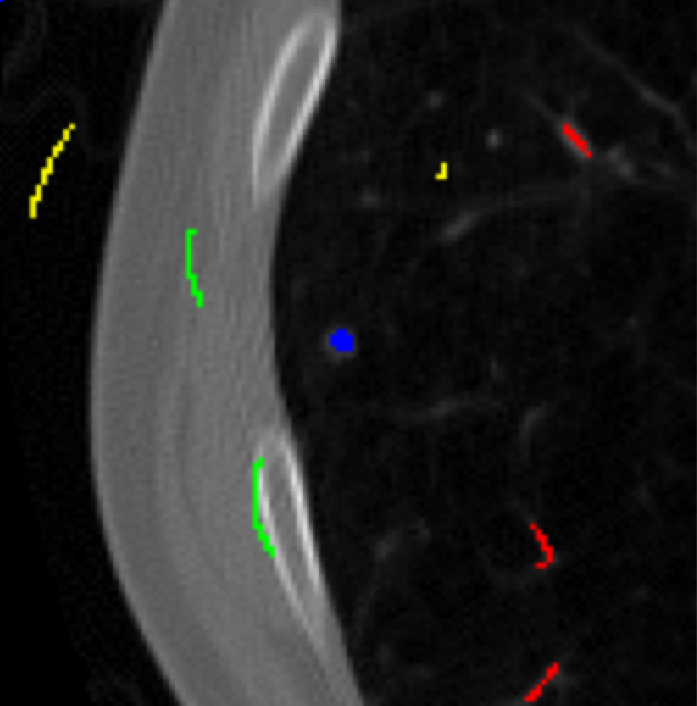
\includegraphics[scale=0.1]{figs/s1.png}}
\subfigure[]{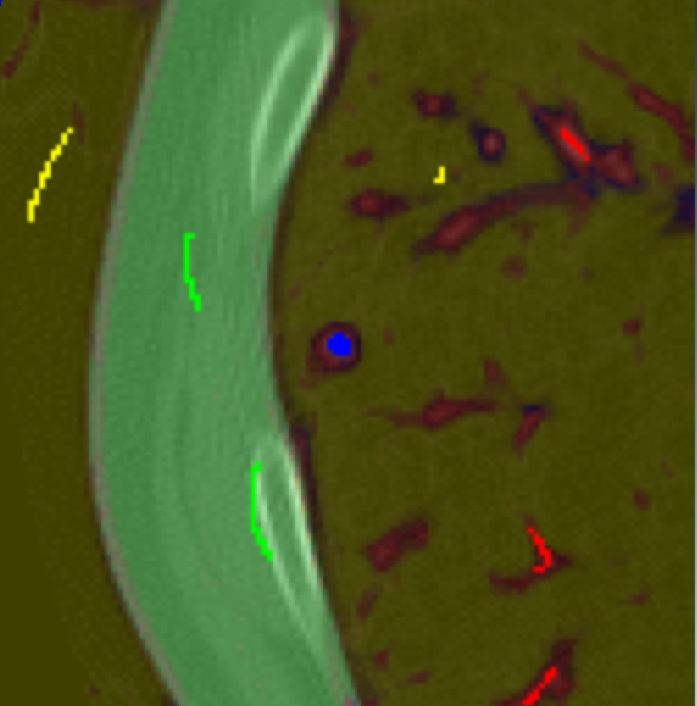
\includegraphics[scale=0.1]{figs/s2.png}}
\subfigure[]{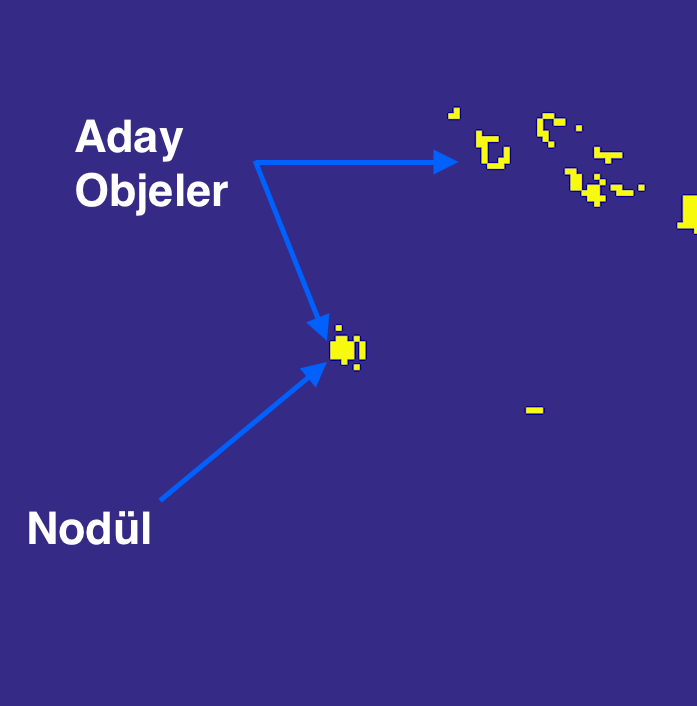
\includegraphics[scale=0.1]{figs/s3.png}}
\caption{a) Etkileşimli öğrenme aracında voksel sınıflandırıcının eğitimi ve kullanıcı tarafından yapılan işaretleme. Sarı: hava boşluğu, kırmızı: damar, yeşil: doku ve kemik; mavi ise nodül sınıflarını göstermektedir. b) Çevrimiçi eğitim sırasında, ilastik'in hesapladığı sınıf olasılıklarının gösterimi. c) Voksel sınıf olasılıklarından çift eşikleme yöntemiyle belirlenen aday objeler.}
\label{fig1}
\end{figure}

\subsection{Aday Belirleme}
Bir önceki aşamada, etkileşimli eğitim tamamlanarak sınıflandırıcı oluşturulduktan sonra, eğitimde kullanılmayan sınama taramalarına uygulandı ve tüm hacimler için voksel/sınıf olasılıkları hesaplandı. Hesaplanan olasılıklardan belirli bir eşik değerini geçenleri aday obje olarak belirlendi. Şekil \ref{pcatch} örnek bir nodül için olasılık haritası görülmektedir, bu değerlerin merkezden uzaklaştıkca azaldığı ve homojen olmadığı görülmektedir. Yüksek olasılıklı voksellere bağlı düşük olasılıklı voksellerin de aday obje maskesinde yer alması için morfolojik geri-çatma ile iki seviyeli bir eşikleme uygulandı. Yüksek ve düşük eşikler sırasıyla $\alpha_1 = 0.6$ ve $\alpha_2 = 0.4$ 'dir. Bu işlemin sonucunda ortaya çıkan ikili maskeden, sırasıyla morfolojik açma işlemi (2x2 basit yapı elemanı) ve bağlı bileşen analizi işlemleri ile aday objeler çıkartıldı.

\begin{figure}[t]
\centering
\subfigure[]{
\includegraphics[height=1.8cm]{figs/probcatch.png}\label{pcatch}}
\subfigure[]{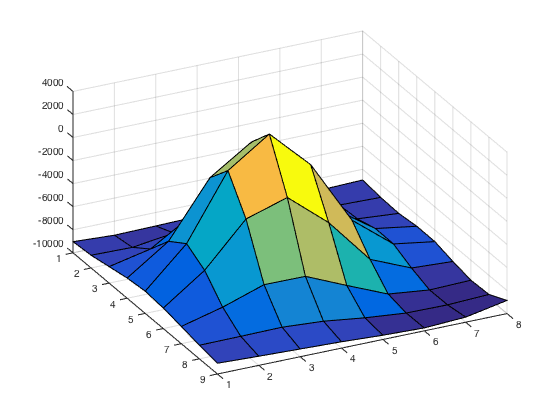
\includegraphics[height=2.5cm]{figs/sum_nod.png}\label{sumnod}}
\subfigure[]{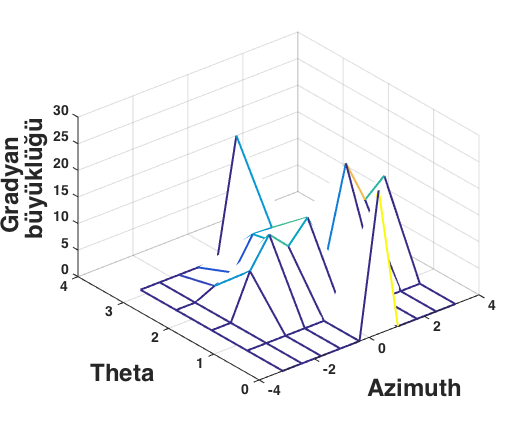
\includegraphics[height=2.5cm]{figs/grad_hist.png}\label{gradhist}}
\caption{a) Olasılık haritasından bir nodül kesiti. Sarı alanlar yüksek, mavi alanlar düşük olasılık değerleridir. b) Bir nodülün z-ekseninde toplanarak oluşturulmuş izdüşümü. c) Gradyan açılarının büyüklük histogramı.}
\label{fig2}
\end{figure}

\subsection{Öznitelik Çıkarımı}\label{oznitelik}
Her bir aday obje ile ilişkili maske ve orijinal BT tarama kullanılarak toplam 18 adet farklı öznitelik vektörü hesaplandı. Bu öznitelikleri genel ve de çalışmamıza özgün olarak iki grupta inceleyebiliriz.

\subsubsection{Genel Öznitelikler}
İlk gurupta, hacim, varsayımsal çap, hacim sınırlayan kutu ölçek oranı, yüzey alanı hacim oranı gibi şekil öznitelikleri vardır. Bu hesaplamalar, Şekil \ref{fig3}'de gösterildiği gibi aday objenin ait olduğu taramadaki ikili maske üzerinden hesaplandı. Bunların yanında maksimum-minimum HU yoğunlukları, 32 bölümlü HU yoğunluk dağılımı (ing. histogram) bulunmaktadır. Bu öznitelikler ise, maskenin orijinal BT taramasındaki izdüşümü üzerinden hesaplandı.

\begin{figure}[tb]
\centering
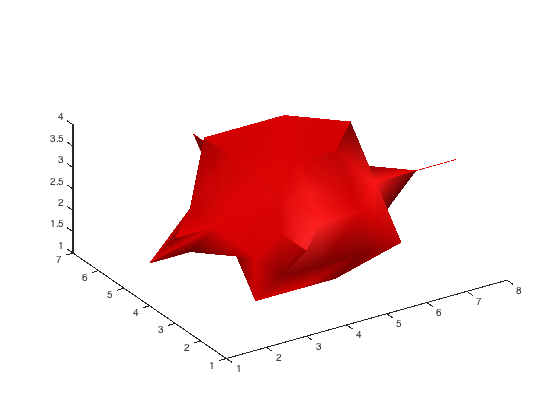
\includegraphics[scale=0.2]{figs/ex_nod.png}
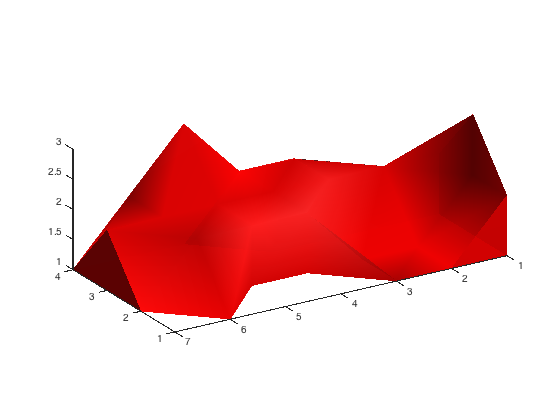
\includegraphics[scale=0.2]{figs/ex_ves.png}
\caption{İkili gösterimde geri çatılmış aday objeler. Solda nodül ve sağda nodül olmayan yapı.}
\label{fig3}
\end{figure}

\subsubsection{Voksel gradyanların açı histogramı özniteliği}
Radyologlar, tomografi taramalarındaki anormaliklerin tespiti için farklı kesitlerdeki değişimleri inceler. Örneğin damarlar farklı kesitlerde konum değişimi gösterirken, anormal yapılar, anatomiden bağımsız lokal değişimler gösterir. Bizde, bu gözlemden yola çıkarak kesitler arasındaki farklılıkları özetleyebilmek için gradyan-oryantasyon-histogramı \cite{dalal2005} özniteliğine benzer "görece daha basit" bir öznitelik oluşturduk. Bu özniteliği çıkartmak için sırasıyla 3 uzamsal boyutta türevleri (\ref{eqg1});
Gradyan büyüklüğünü (\ref{eqg2}) ve 3 boyutta küresel açılarını ($\theta, \phi$) (\ref{eqg3}) hesaplandı.

\begin{equation}
\nabla f = <\frac{\partial f}{\partial x} (x,y,z),
			\frac{\partial f}{\partial y} (x,y,z),
			\frac{\partial f}{\partial z} (x,y,z)>
\label{eqg1}
\end{equation}

\begin{equation}
M(x, y, z) = \sqrt{\frac{\partial f}{\partial x}^2 + \frac{\partial f}{\partial y}^2 + \frac{\partial f}{\partial z}^2}
\label{eqg2}
\end{equation}

\begin{equation}
\theta(x, y, z) = \frac{\cos^{-1}(\frac{\partial f}{\partial z})}{M(x, y, z)}, \phi(x, y, z) = \tan^{-1}(\frac{\frac{\partial f}{\partial x}}{\frac{\partial f}{\partial y}})
\label{eqg3}
\end{equation}

$\theta$ ve $\phi$ açılarının yönlerine göre dağılım grafikleri, $M(x, y, z)$ değerleri ağırlığınca hesaplandı ve $L_2$ \cite{dalal2005} normalizasyonu uygulandı. Şekil \ref{gradhist}, örnek bir histogram görülebilir. Ayrıca gradyan büyüklüğü $M(x, y, z)$, her üç eksende de toplanarak 2 boyuttaki izdüşümlerini hesaplandı (\ref{g21}). Bu izdüşümler üzerinde tekrar gradyan hesaplanarak (\ref{g22}) -ikinci türeve benzeşen- kesitler arası değişim bilgisi gösterime eklendi. Son olarak, gradyan açıları hesaplanarak (\ref{g23}) 1-boyutlu açı histogramları hesaplandı.
 
 \begin{equation}
 p^{M_x} = \sum_x{M}, \quad
 p^{M_y} = \sum_y{M}, \quad
 p^{M_z} = \sum_z{M}, \quad
\label{g21}
\end{equation}

\begin{equation}
\nabla p^{M_i} = <\frac{\partial p^{M_i}}{\partial x} (x,y),
			\frac{\partial p^{M_i}}{\partial y} (x,y)
\label{g22}
\end{equation}

\begin{equation}
L(x, y) = \sqrt{\frac{\partial p^{M_i}}{\partial x}^2 + \frac{\partial p^{M_i}}{\partial y}^2}
\label{g23}
\end{equation}

\subsubsection{İki boyutlu Gaussian uydurma}
Yine aday objenin yerel mi, yoksa anatomik bir uzantı olup olmadığını yakalamak için HU yogunluğunun z-y, x-z, y-z düzlemlerindeki izdüşümlerini kullanmaktayız. Bu amaçla, izdüşümleri hesaplanıp 2 boyutlu bir Gaussian fonksiyona uyduruldu. Uydurma katsayıları öznitelik olarak kullanıldı. Şekil \ref{sumnod}, örnek bir izdüşümün görülmektedir. Eğer aday obje yerel ise (Örneğin damar değilse) izdüşümü bir Gaussian'a benzeyecektir. Öte yanda, anatomik yapıların izdüşümleri kesitlerin arasında hareketli olduğundan izdüşümleri Gaussian'dan uzaklaşacaktır. 
Kullandığımız model aşağıda görülmektedir: 
\begin{equation}
v_1 = \frac{((X-c_1) * \cos(t_1) + (Y-c_2) * \sin(t_1))}{w_1}
\label{eq1}
\end{equation}
\begin{equation}
v_2 = -\frac{((X-c_1) * \sin(t_1) + (Y-c_2) * \cos(t_1))}{w_2}
\label{eq2}
\end{equation}
\begin{equation}
Z = f(X, Y) = a + b * e({-v_1}^2 - {v_2}^2))
\label{eq3}
\end{equation}
Yukarıda (\ref{eq3})'da belirtilen, $X, Y$ vektörleri 2 boyutlu yüzey alanını temsil eder ve bağımsız değişkenlerdir. $Z$ ise yüzeyin üzerindeki HU yoğunluklarını içeren vektördür. $\lambda = \lbrace a, b, c_1, c_2, t_1, w_1, w_2 \rbrace$ katsayıları, öznitelik olarak kullanılmak üzere her bir aday için hesaplandı.

\subsection{Rastgele Karar Ormanı}
Obje sınıflandırıcısı olarak scikit\footnote{scikit-learn.org/} kütüphanesinden (ing. Random Forest) rastgele karar ormanı sınıflandırıcısını seçildi. Eğitim kümemizi öznitelikler ve etiket çiftleri oluşturmaktadır: $T = \lbrace (\vec{x_1}, y_1), (\vec{x_2}, y_2), .., (\vec{x_n}, y_n) \rbrace$. Öznitelik vektörü $\vec{x_i}$, bütün özniteliklerinin peşpeşe eklenmesinden oluşur.

\section{DENEYLER}

\subsection{Doğruluk Kriteri}
Veri 1 ve 2 kümelerine ait nodüllerin orta konum noktaları bulunmaktadır. Nodül olarak sınıflandırılan bir aday objenin doğru sayılabilmesi için uzman tarafından işaretlenmiş bir konum orta noktasının, aday objenin hacmiyle örtüşmesi gerekmektedir. Doğru tespit edilen nodüllerin elle işaretlenen toplam nodüllerin sayısına oranı \textbf{doğru tespit} oranını verir. Öte yandan, nodül olarak sınıflandırılmış ancak uzman işaretleriyle örtüşmeyen objeler \textbf{yanlış tespit} olarak sayılmaktadır. Toplam yanlış tespitlerin, tarama sayısına bölünmesiyle tarama başına \textbf{ortalama yanlış tespit sayısı} bulunmaktadır.

%Bu kriter, Anode09\cite{anode}'da kullanılan yarı çapın 1.5 katı kadar yakın olma kriterinden daha yakındır.
\subsection{Eğitim}
Bölüm \ref{veriler}'de anlatılan Veri-1 kümesini eğitim, Veri-2 kümesini ise anlık sınamalarımız ve doğrulama işlemlerimiz için ayrıldı. Voksel olasılıklarının öğrenilmesi için ilastik \cite{sommer2011} programının eğitilmesi Bölüm \ref{ilastik}'de açıklanmıştır. Aday objelerin sınıflandırılması için ise, Veri 1 kümesindeki toplam 67 taramadan gelen 228 nodül ve bu taramalardan rastgele seçilmiş 3000 adet nodül olmayan obje ile rasgele karar ormanı eğitilmiştir.

\subsection{Sınama}
Sınamalar için Anode09 yarışmasında etiketsiz olarak verilen 50 adet deney kümesi (Veri 3) kullanıldı. Her biri $512x512xN$ büyüklüğünde olan bu taramalardaki nodüllerin konumları bize verilmemiştir. Bu taramaların tümünü aday obje belirleme işleminden geçirdikten sonra tarama başına yaklaşık 900 aday obje otomatik olarak tespit edildi. Her aday obje için öznitelikler çıkarıldı ve sınıflandırıcıya sokuldu. Sınıflandırıcının ürettiği nodül olma olasılıkları farklı eşik değerlerinde eşiklenerek farklı doğruluk ve tarama başına ortalama yanlış tespit oranları elde edildi: FROC analizi yapıldı. Anode09\cite{anode09}'da olduğu gibi bizde tarama başına ortalama yanlış tespit oranları 1/8, 1/4, 1/2, 1, 2, 4 ve 8 için doğruluk oranlarını hesaplandı. Önerdiğimiz sistemin FROC grafiği incelendiğinde ortalama 8 yanlış tespite 0.52 doğrulukta doğru tespit yaptığı gözlemlenmiştir. Şekil \ref{evalfeas} farklı boyutlardaki nodüllerin tespit oranlarını göstermektedir. Büyük nodüllerin sistemimiz tarafından daha az hassasiyette yakalandıkları gözlemlenmektedir. Bunun nedeni interaktif öğrenme aşamasındaki eğitim kümemizde büyük nodüllerden sadece 2 adet örnek olmasıdır.

Anode09 yarışmasında değerlendirilen en iyi altı sistem A, B, C, D, E ve F sistemleridir. Şekil \ref{eval}'da, FROC eğrileri ile sonuçlarımızın diğer sistemlerle karşılaştırılması sunulmuştur. Yöntemimizin, yarışmadaki değerlendirme kriterlerine göre ilk 6 sistemin sıralamasına girebildiği; ve ortalama 8 yanlış pozitife çıkıldığında en duyarlı üçüncü yöntem olduğu gözlenebilir.

\begin{figure}[tb]
\centering
\subfigure[]{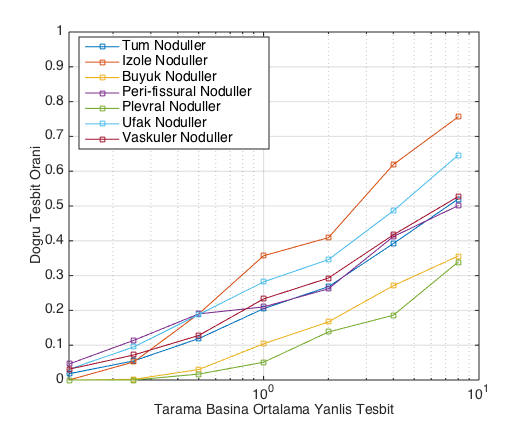
\includegraphics[height=5cm]{figs/nodule_type_detections.png}\label{evalfeas}}
\subfigure[]{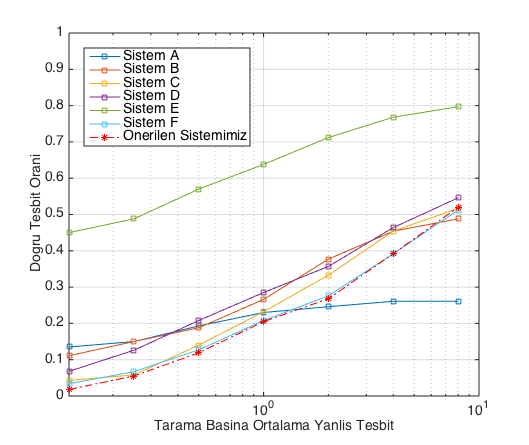
\includegraphics[height=5cm]{figs/eval2.png}\label{eval}}
\caption{a) Önerdiğimiz yöntemin Anode09'da farklı tip ve boyutlardaki nodüller için FROC eğrileri. b) bütün nodül tiplerine göre diğer sistemlerle karşılaştırması.}
\end{figure}

\section{SONUÇLAR}
Bu çalışmada, akciğer BT taramalarında nodül tespitine yönelik yeni ve özgün bir yöntem sunulmuştur. Yöntemimiz, akciğer organına ve nodül görünümüne özelleşmiş herhangi bir ön kabulde bulunmamaktadır. Bu yönüyle, literatürde yer alan diğer yaklaşımlardan oldukça farklıdır. Bir önbölütlemeye ihtiyaç duymadan akciğer organında farklı tipteki nödülleri tespit edebilmektedir. Anode09 örnek veri kümesinde yaptığımız sınamalarda aldığımız nodül tespit sonuçları, yarışmada ilk altıya giren algoritmalarla karşılaştırılabilir düzeydedir. Ancak algoritmanın büyük nodüllerde yeterli başarıyı gösteremediği gözlenmiştir. Bu eksikliği gidermek için eğitim kümesi zenginleştirelecektir. 

% An example of a floating figure using the graphicx package.
% Note that \label must occur AFTER (or within) \caption.
% For figures, \caption should occur after the \includegraphics.
% Note that IEEEtran v1.7 and later has special internal code that
% is designed to preserve the operation of \label within \caption
% even when the captionsoff option is in effect. However, because
% of issues like this, it may be the safest practice to put all your
% \label just after \caption rather than within \caption{}.
%
% Reminder: the "draftcls" or "draftclsnofoot", not "draft", class
% option should be used if it is desired that the figures are to be
% displayed while in draft mode.
%
%\begin{figure}[!t]
%\centering
%\includegraphics[width=2.5in]{myfigure}
% where an .eps filename suffix will be assumed under latex,
% and a .pdf suffix will be assumed for pdflatex; or what has been declared
% via \DeclareGraphicsExtensions.
%\caption{Simulation Results}
%\label{fig_sim}
%\end{figure}

% Note that IEEE typically puts floats only at the top, even when this
% results in a large percentage of a column being occupied by floats.

% An example of a double column floating figure using two subfigures.
% (The subfig.sty package must be loaded for this to work.)
% The subfigure \label commands are set within each subfloat command, the
% \label for the overall figure must come after \caption.
% \hfil must be used as a separator to get equal spacing.
% The subfigure.sty package works much the same way, except \subfigure is
% used instead of \subfloat.
%
%\begin{figure*}[!t]
%\centerline{\subfloat[Case I]\includegraphics[width=2.5in]{subfigcase1}%
%\label{fig_first_case}}
%\hfil
%\subfloat[Case II]{\includegraphics[width=2.5in]{subfigcase2}%
%\label{fig_second_case}}}
%\caption{Simulation results}
%\label{fig_sim}
%\end{figure*}
%
% Note that often IEEE papers with subfigures do not employ subfigure
% captions (using the optional argument to \subfloat), but instead will
% reference/describe all of them (a), (b), etc., within the main caption.


% An example of a floating table. Note that, for IEEE style tables, the
% \caption command should come BEFORE the table. Table text will default to
% \footnotesize as IEEE normally uses this smaller font for tables.
% The \label must come after \caption as always.
%
%\begin{table}[!t]
%% increase table row spacing, adjust to taste
%\renewcommand{\arraystretch}{1.3}
% if using array.sty, it might be a good idea to tweak the value of
% \extrarowheight as needed to properly center the text within the cells
%\caption{An Example of a Table}
%\label{table_example}
%\centering
%% Some packages, such as MDW tools, offer better commands for making tables
%% than the plain LaTeX2e tabular which is used here.
%\begin{tabular}{|c||c|}
%\hline
%One & Two\\
%\hline
%Three & Four\\
%\hline
%\end{tabular}
%\end{table}


% Note that IEEE does not put floats in the very first column - or typically
% anywhere on the first page for that matter. Also, in-text middle ("here")
% positioning is not used. Most IEEE journals/conferences use top floats
% exclusively. Note that, LaTeX2e, unlike IEEE journals/conferences, places
% footnotes above bottom floats. This can be corrected via the \fnbelowfloat
% command of the stfloats package.


% use section* for acknowledgement
%\section*{TEŞEKKÜR}
%Yazarın teşekkür etmek istediği kurum yada kişiler burada belirtilecek.

% trigger a \newpage just before the given reference
% number - used to balance the columns on the last page
% adjust value as needed - may need to be readjusted if
% the document is modified later
%\IEEEtriggeratref{8}
% The "triggered" command can be changed if desired:
%\IEEEtriggercmd{\enlargethispage{-5in}}

% references section

% can use a bibliography generated by BibTeX as a .bbl file
% BibTeX documentation can be easily obtained at:
% http://www.ctan.org/tex-archive/biblio/bibtex/contrib/doc/
% The IEEEtran BibTeX style support page is at:
% http://www.michaelshell.org/tex/ieeetran/bibtex/
%\bibliographystyle{IEEEtran}
% argument is your BibTeX string definitions and bibliography database(s)
%\bibliography{IEEEabrv,../bib/paper}
%
% <OR> manually copy in the resultant .bbl file
% set second argument of \begin to the number of references
% (used to reserve space for the reference number labels box)

\bibliographystyle{IEEEtran}

\begin{thebibliography}{1}

\bibitem{anode09}
Ginneken Bram van, Samuel G. Armato III, Bartjan de Hoop, et al, 2010.  Comparing and combining algorithms for computer-aided detection of pulmonary nodules in computed tomography scans: The ANODE09 study, Medical Image Analysis, vol 6., 2010

\bibitem{ferlay2012}
Ferlay J, Soerjomataram I, Ervik M, Dikshit R, et al. GLOBOCAN 2012 v1.0, Cancer Incidence and Mortality Worldwide: IARC CancerBase No. 11 [Internet], 2012.

\bibitem{rubin2015}
Rubin, G. D. Lung Nodule and Cancer Detection in Computed Tomography Screening. Journal of thoracic imaging, 30(2), 130-138, 2015.

\bibitem{lidc2011}
Armato III, S. G., McLennan, G., Bidaut, L.,et al. The lung image database consortium (LIDC) and image database resource initiative (IDRI): a completed reference database of lung nodules on CT scans. Medical physics, 38(2), 915-931, 2011.

\bibitem{sommer2011}
Sommer, C. , Straehle, C. , Kothe, U. and Hamprecht F.A. ilastik: Interactive learning and segmentation toolkit. In IEEE Biomedical Imaging (ISBI), 203-233, 2011.

\bibitem{tek2014}
Tek, F. B., Kroeger, T., Mikula, S.,\& Hamprecht, F. A. “Automated cell nucleus detection for large-volume electron microscopy of neural tissue”. In IEEE Biomedical Imaging (ISBI), pp 69-72, 2014.


\bibitem{dalal2005}
Dalal, N.; Triggs, B., "Histograms of oriented gradients for human detection," in Computer Vision and Pattern Recognition, 2005. CVPR 2005. IEEE Computer Society Conference on , vol.1, no., pp.886-893 vol. 1, 25-25 June 2005.

\end{thebibliography}

% that's all folks
\end{document}
